\documentclass{amsart}
\usepackage{graphicx}
\usepackage{booktabs}
\usepackage{multirow}
\usepackage{hyperref}
\usepackage{float}

\title{Influence of Cholesterol upon Heart Disease (Geometric Sampling)}
\author{Eric S. Wright}
\begin{document}
\begin{abstract}
Heart disease is often linked to many different factors that are tied to lifestyle, genetics, physiology, etc. It is widely believed that high cholesterol is a major causal influence for heart disease. In this article,we investigate what this might mean in practice. Specifically, we set out to determine if the well-known, publicly-available Cleveland data set on heart disease in medical study subjects supports the notion that subjects with high cholesterol will be more prone to developing heart disease. We approach this problem by applying a geometric sampling methodology to the Cleveland data set. We repeatedly sample one subject at a time with high cholesterol levels from the data set (with replacement)and record the number of healthy subjects we observe before encountering our first subject with heart disease. Each time we perform this task adds a data point to our control data set. Then we apply the same process to the test subjects in the data set with normal cholesterol counts in order to build our experimental data set. Finally, we apply selected hypothesis tests to our samples to determine if the heart disease counts in the high cholesterol group are significantly different from the heart disease counts taken from the moderate cholesterol subjects.
\end{abstract}
\maketitle
\section{Introduction}\label{S:Introduction}
We address the question of how significant the relationship between high cholesterol and heart disease is by first obtaining the publicly available Cleveland heart disease data set. This data set is curated by the UCI machine learning repository and can be found at \url{https://archive.ics.uci.edu/ml/datasets/heart+disease}. The data consists of over 300 records of medical test subjects that summarize multiple risk factors for heart disease that include cholesterol level. The data also indicates whether or not each subject developed heart disease. We repeated a process 50 times in which we sample one subject at a time with high cholesterol levels from the data set (with replacement)and record the number of healthy subjects we observe before encountering our first subject with heart disease. Then, we performed the same task 50 times on the test subjects with normal cholesterol. These counts produced the following control and experimental data sets respectively:
\begin{align*}
D_{control}=\{&1, 8, 0, 1, 0, 4, 4, 1, 0, 0, 0, 2, 0, 1, 0, 0, 2, 3, 2, 1, 1, 0, 0, 0, 0,\\
&2, 1, 2, 1, 0, 0, 0, 4, 0, 3, 0, 1, 1, 1, 0, 2, 0, 2, 0, 0, 0, 3, 0, 2, 1
\}
\end{align*}
and
\begin{align*}
D_{experimental}=\{&3, 3, 6, 0, 2, 2, 1, 0, 0, 0, 0, 1, 5, 0, 0, 5, 4, 1, 2, 1, 0, 0, 0, 0, 0,\\
&1, 1, 2, 4, 2, 0, 1, 0, 3, 2, 0, 0, 0, 5, 3, 1, 0, 0, 3, 0, 5, 6, 7, 1, 0
\}.
\end{align*}
We expect that there will be a link between normal cholesterol and a reduced risk of heart disease. Throughout the remainder of this article, we will evaluate this expectation by fitting a geometric model to $D_{control}$, validating the fit, and then performing a selection of hypothesis tests aimed at determining if there is a significant difference between the data in $D_{experimental}$ and what the geometric model leads us to expect or if there is a significant difference between the two data sets themselves.

\section{Data Analysis and Visualization}
Before fitting a model to $D_{control}$, we computed summary statistics of central tendency, extent, variability, asymetry, and importance of outliers for the data set. These are reported in table \ref{Tbl:statistics}.
\begin{table}[h]
\centering
\begin{tabular}{lr}
\toprule
\multicolumn{2}{c}{\textbf{Summary Statistics of $D_{control}$}}\\
\midrule
Mean & 1.14 \\
Median& 1\\
Mode& 0\\
Max& 8\\
Min& 0\\
Range& 8\\
StdDev& 1.5364\\
Variance& 2.3604\\
Quartiles& 0, 1, 2\\
IQR& 2\\
Skewness& 2.1139\\
Bowley& 0\\
Kurtosis& 8.9544\\
\bottomrule
\end{tabular}
\caption{Summary statistics of healthy test subject counts sampled geometrically from the high cholesterol group.\label{Tbl:statistics}}
\end{table}
Our summary statistics begin to tell a story about our control data set. All measures of central tendency are relatively similar to each other. The positive skewness suggests that the data is right skewed, but this is expected of geometric data. The large value of kurtosis indicates that there might be outliers present.

We can see these features within the control data by looking at visualizations. The asymmetric nature and outliers in the high range of our data are apparent in both our box and whisker plot (see figure \ref{F:boxplotfinal}) and our histogram (pictured in figure \ref{F:absoluteFrequencies}).
\begin{figure}
\centering
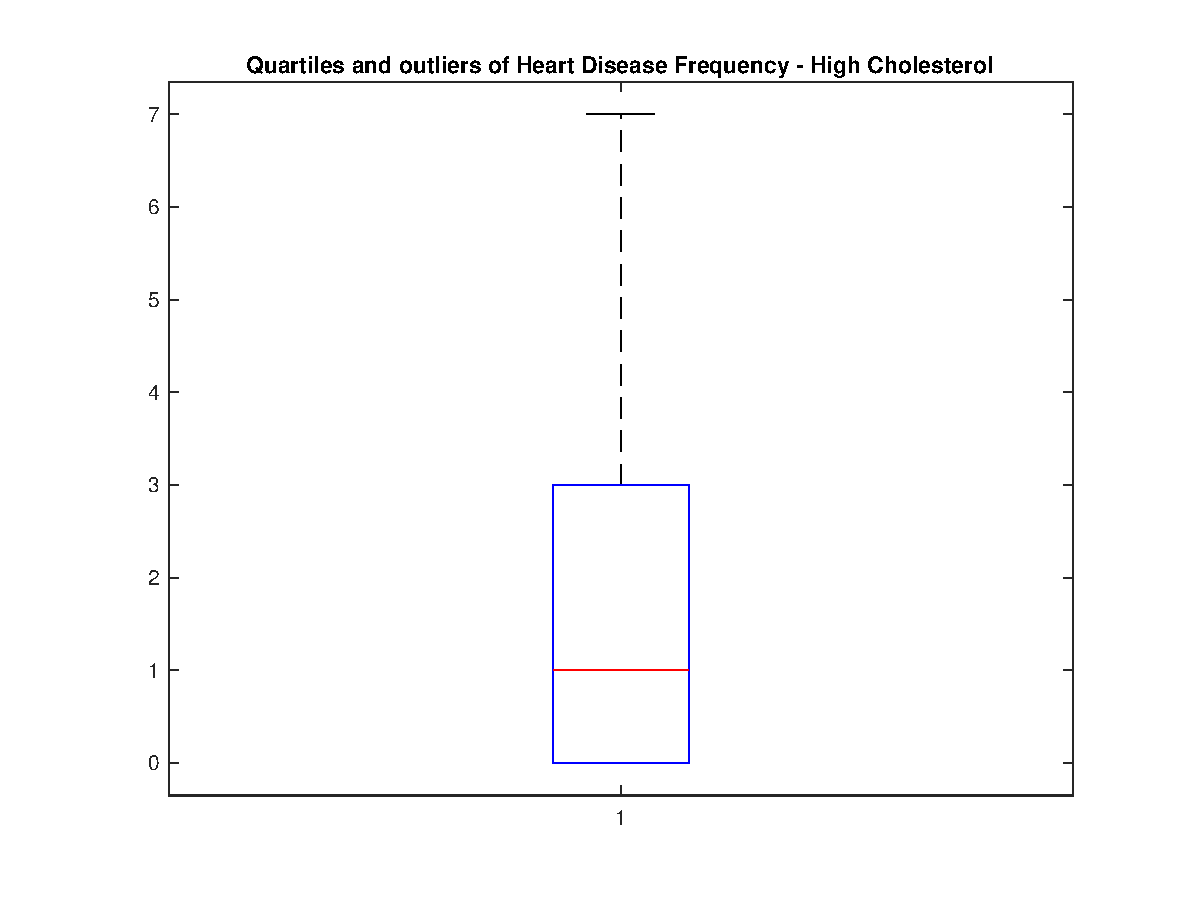
\includegraphics[scale=0.55]{boxplotfinal}
\caption{Box and whisker plot of heart disease control data.\label{F:boxplotfinal}}
\end{figure}

\begin{figure}
\centering
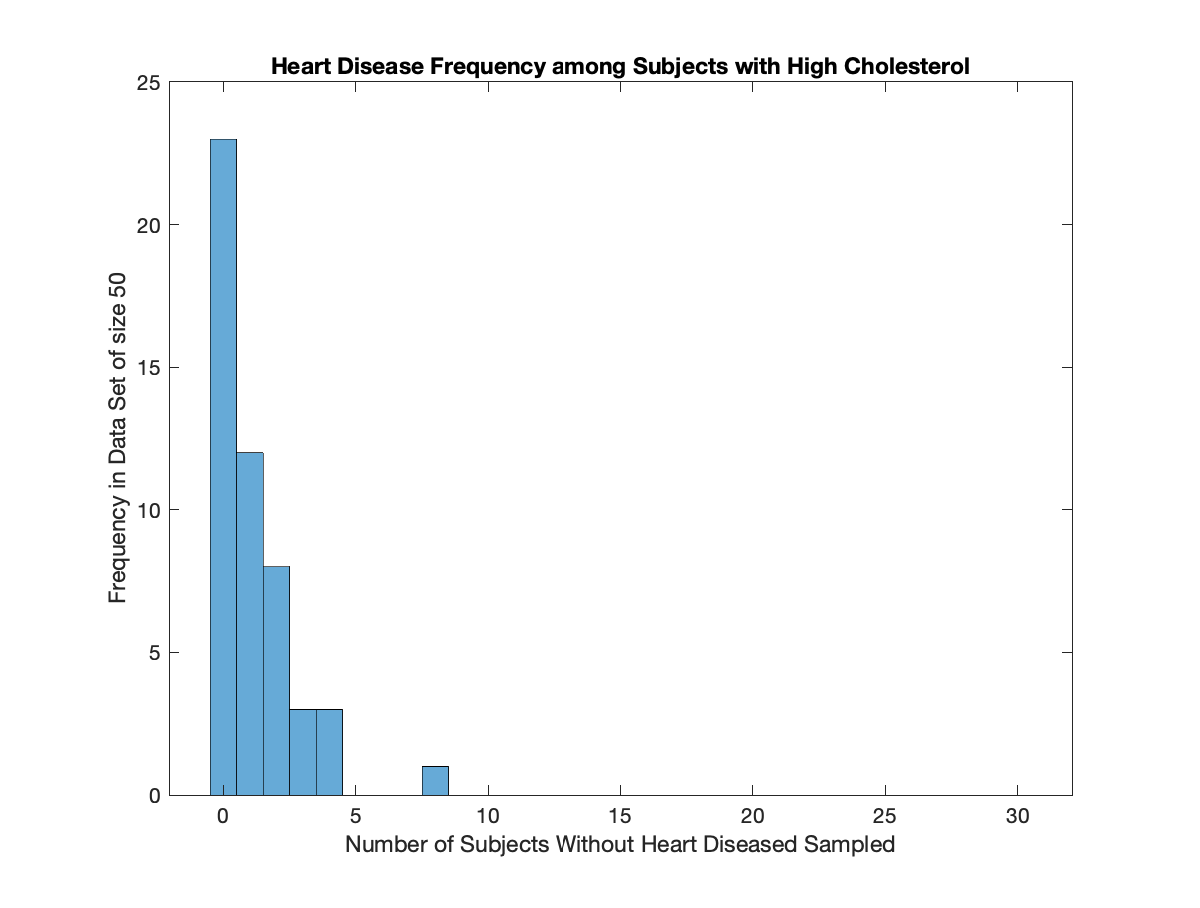
\includegraphics[scale=0.55]{histogramfinal}
\caption{Absolute frequencies of control data.\label{F:absoluteFrequencies}}
\end{figure}

\section{A Model for Data Collection}
We built our control data set by counting the lengths of 50 randomly selected subjects of healthy test subjects that we observed before encountering our first test subject with heart disease. Each subject in each sequence was collected with replacement from the Cleveland data set. It is reasonable to assume that the one test subject's tendency to develop heart disease is independent from that of any other test subject, so we model our control data with a geometric framework. Our data can (in principle) take on any integer value ranging over all non-negative integers, so our sample space is the set $$\Omega=\{x: 0\le x< \infty\},$$  where $x$ represents the number of healthy subjects we encountered in a sequence before the first test subject with heart disease. This sample space is countably infinite. We may organize the measurable events of our probability space into a $\sigma$-algebra $S$ by forming the power set, or set of all subsets, of the sample space.  There will be an uncountably inffinite number of events in $S$. Finally, the geometric framework uses the geometric distribution to assign probabilities to the outcomes in $\Omega$:
\[
G(p;x)=p(1-p)^x.
\]
Here, $p$ represents the probability that any given test subject will develop heart disease. This distribution predicts the probability of observing any value $x$ from our sample space. We may use it to compute the probability of any event $E$ in $S$ by summing the probabilities of each outcome in $E$:
\[
P(E)=\sum_{x\in E} G(p;x).
\]
As such, the geometric distribution generates the probability measure of the probability space that models our data collection approach. However, in order to make use of this distribution in this way, we will need to be able to measure or estimate the unknown parameter $p$.
\section{Derivation of a Theoretical Distribution through Parameter Estimation}
As already stated, in order to model our data collection with the geometric distribution, we will need to estimate the parameter $p$. Recall $p$ represents represents the probability that any given test subject will develop heart disease. We estimated $p$ by applying maximum likelihood estimation to $D_{control}$. This resulted in the value
\[
p\simeq 0.4673.
\]
Next, we turn to validating the geometric model with this parameter value using both qualitative and quantitative techniques. If we plot the graph of expected frequencies predicted by this theoretical distribution on the same axes as the histogram of our control data (see figure \ref{F:graphicalAssessement}), we can see that the observed freqeuencies found in the control data appear to be quite similar to the expected frequencies. So far, this indicates good, qualitative agreement between the model and the control data.
\begin{figure}
\centering
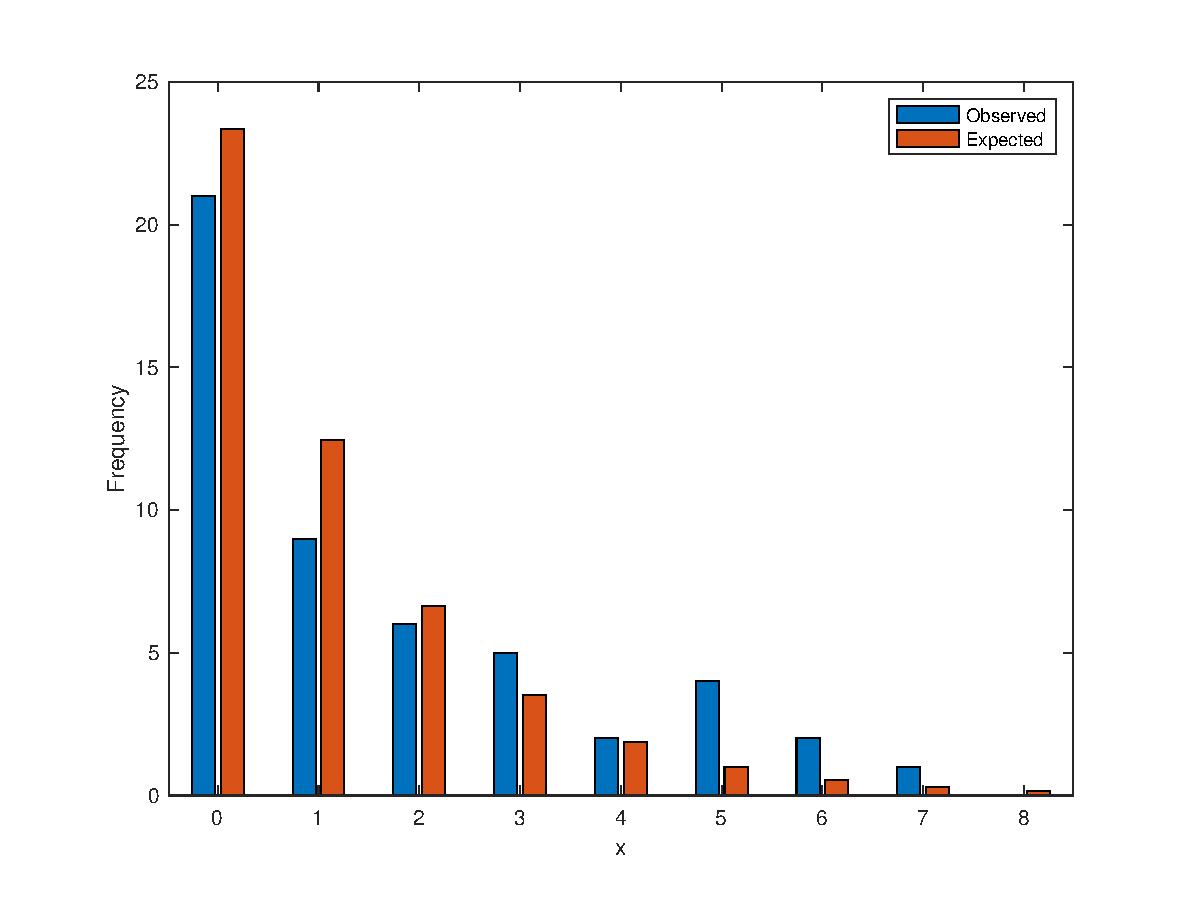
\includegraphics[scale=0.55]{histvalidationfinal}
\caption{
Comparison between empirical relative frequencies and theoretical: geometric model.\label{F:graphicalAssessement}}
\end{figure}
We can also assess the fit of our model to the control data by computing the theoretical values of mean, variance, skewness, and kurtosis of our geometric model and comparing them to the values we have already computed for our control data set. This comparison is summarized in Table \ref{Tbl:quantitativeAssessment}.
\begin{table}
\begin{tabular}{lrrrr}
\toprule
			&	{\bf Mean}	&	{\bf Variance}	&	{\bf Skewness}	&	{\bf Kurtosis}\\\midrule
{\sl Empirical}	&	1.14 	&	2.3604	&	2.1139	&	8.9544\\ 
{\sl Theoretical}&	1.14    & 	2.4396	&	2.1000		&	9.4099\\
\bottomrule
\end{tabular}
 \caption{Quantitative comparison of the theoretical shape parameters of the geometric model distribution to the empirical shape parameters of the control data set.\label{Tbl:quantitativeAssessment}}
\end{table}

Again, agreement between the empirical and theoretical shape parameter values is rather close, so we continue to build evidence in favor of retaining the geometric model for $D_{control}$.

Another fit assessment we can perform is to construct a quantile-quantile plot, or QQ plot, in which we plot the quantiles of each data point in $D_{control}$ against the theoretical quantiles of the geometric distribution. When the distribution fits the data well, the QQ plot should show a linear relationship between the empirical and theoretical quantiles. Our QQ plot is displayed in figure \ref{F:qqplot}, and it is evident that such a linear relationship exists. The QQ plot provides more evidence in favor of a good fit between the binomial model and the control data.
\begin{figure}
\centering
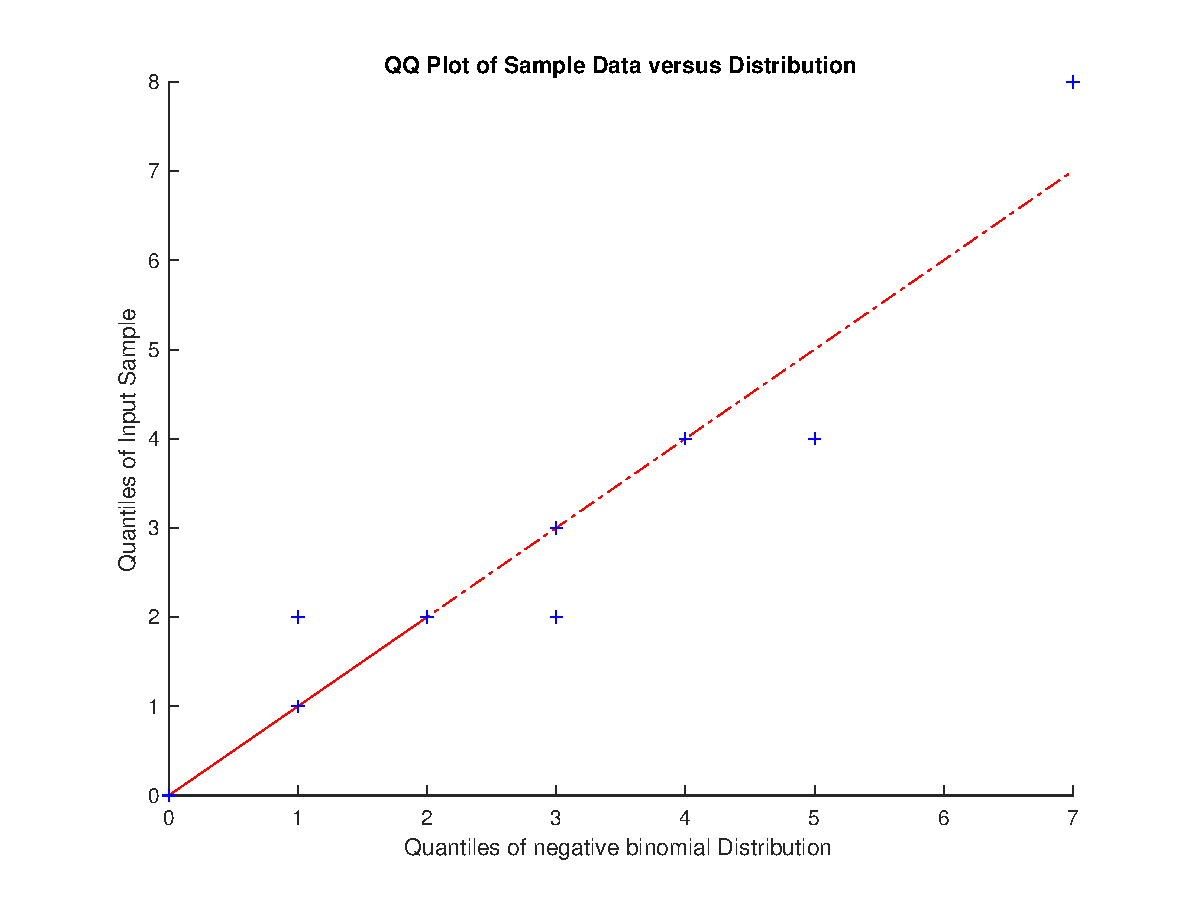
\includegraphics[scale=0.55]{qqplotfinal}
\caption{
Quantile-quantile plot expressing the relationship between the observed quantiles of each point in $D_{control}$ and the theoretical quantiles of the geometric distribution.\label{F:qqplot}}
\end{figure}

Finally, we can be more quantitative still in comparing the data to the geometric model by performing a goodness of fit test.  To do so, we pool the possible values from the sample space into bins that ensure there is an expected frequency ($E$) (predicted by the geometric distribution) of at least 5 observations per bin.  Then, we compare these predictions to the actual frequencies observed ($O$) in these bins in our data set.  This information is summarized in the Table \ref{Tbl:chi2}.

\begin{table}
{\footnotesize
\begin{tabular}{lcccccc}
\toprule
\multirow{2}{*}{Frequencies} & \multicolumn{4}{c}{Bins}\\	
	& $0\le x < 1$ &	$1\le x <2$ & 	$2\le x <3$ & $3\le x< \infty$\\
	\midrule
Observed& 23& 12 & 8 & 7\\
Expected & 23.3645 & 12.4465 & 6.6304 & 7.5586 \\
\bottomrule
\end{tabular}}
\caption{Expected and observed frequencies for Pearson's goodness of fit test..\label{Tbl:chi2}}
\end{table}

From this data, we may compute the $\chi^2$ test statistic.
$$\chi^2=\sum\frac{(E(x)-O(x))^2}{E(x)}=0.3459$$
In order to compare this to an appropriate chi squared distribution, we need to determine the number of degrees of freedom for the comparison of our frequencies.  We have organized our frequencies into 3 bins.  However, in order to compute the expected frequencies, we used the geometric distribution with an estimated value for $p$.  We also are assigning three frequency counts out of a total of 50 observations to three bins. This means that there are $\nu$=4 bins-1 estimated parameter-1 dependency=2 degrees of freedom. According to the $\chi^2$ distribution with $\nu=2$ degrees of freedom, the probability of observing a $\chi^2$ statistic at least as high as ours is
$$P(\chi^2\ge 0.3459;\nu=2)=0.8412.$$
This value is not small enough to reject the null hypothesis that states our model fits our control data well, so we conclude that the expected frequencies predicted by the geometric distribution fit the data we've collected adequately. All of our approaches to validating our geometric model seem to agree that it fits our control data well.
\section{Hypothesis Testing: Impacts of Seasonality upon Earthquake Frequency}
Our aim has been to determine if there is a relationship between cholesterol and heart disease risk in medical test subjects. In particular, we hoped to determine if, when sampling sequences of test subjects with replacement, there is a significant difference in the number of healthy subjects we observe before encountering our first subject with heart disease when we consider subjects who have normal cholesterol levels vs. those who have high cholesterol levels. We successfully devised a geometric model for our control data (the heart disease counts among the subjects with high cholesterol levels). It adequately describes the expected behavior of our control population in hypothesis tests such as the geometric test or the one sample t test, so we will definitely make use of those techniques. However,  we will also make use of tests that look for differences between statistics of the control and experimental samples themselves, such as the two sample t test and a test for differences between two bootstrap samples.

The geometric test is for determining if there is a significant difference between the values in $D_{experimental}$ and what the geometric model leads us to expect within $D_{control}$. The null hypothesis for this test is:
\begin{description}
\item[$H_{0,G}$ (Null Hypothesis)] There is no significant difference between the values in $D_{experimental}$ and the behavior the geometric model leads us to expect within $D_{control}$.
\end{description} 
We applied it to our experimental data in order to test for significant increases in the data relative to the expected behavior predicted by the model (it is only possible to reliably test for increases with the geometric distribution). The test for an increase resulted in only seven of the fifty $P$ values falling below the 5\% threshold. This is a little more than we should expect so see by chance, but by itself, this doesn't seem like an overly compelling result. 

We turn our attention to the one sample t-test for determining if there is a significant difference between the mean of the experimental data set and the theoretical mean predicted by the geometric model. The null hypothesis for this test is
\begin{description}
\item[$H_{0,T}$ (Null Hypothesis)] There is no significant difference between the mean of the experimental data and the theoretical mean of the control population predicted by the geometric model.
\end{description}
The one sample t-test produces a $P$ value of $P=0.0701$. This $P$ value is small, but it isn't below the 5\% threshold that would typically indicate evidence for rejecting $H_{0,T}$. In addition, it provides us with a 95\% confidence interval for the true location of the mean of the population the experimental data was sapled from. This is $1.0957 \le \mu_E \le 2.2243$. Notice that this interval contains the theoretical mean for the control data ($\mu_C=1.14$). This is all indicative of an insignificant difference between the experimental and theoretical mean.

Similarly, the two sample t-test for determining if there is a significant difference between the means of the experimental and control data sets has at least three advantages for our application. First, this approach does not require us to assume any knowledge of the theoretical mean (or the corresponding theoretical distribution) of the population the control data set was sampled from. Second, the two sample t-test is a little more conservative than the one sample test, so if are able to establish significance with it, then we are doing so in a rather grounded way. Finally, the two sample gives us the option of relaxing any assumptions about the equality between the variances of the  experimental and control populations. We don't have any \textsl{a priori} knowledge of whether those variances are similar, but we can check by applying the F test to our control and experimental sample. This results in a p value of $p_F=0.0876$ for evaluating the null hypothesis:
\begin{description}
\item[$H_{0,F}$ (Null Hypothesis)] There is no significant difference between the variance of the experimental data set and the variance of the control data set.
\end{description}.
Since $p_F$ is slightly above a threshold of 5\%, we may retain $H_{0,F}$ and proceed with the two sample t-test for determining if there is a difference between means of two samples. While we would be somewhat justified in assuming the samples have equal variance, we will still make use of the two-sample t-test for samples of unequal variance because it is slightly more conservative. The null hypothesis for the two sample t-test is
\begin{description}
\item[$H_{0,T}$ (Null Hypothesis)] There is no significant difference between the means of the experimental and control data sets.
\end{description}
When we applied the two sample t-test to our control and experimental samples, we achieved a p-value of $p_T=0.1480$, so we again have insufficient evidence for rejecting $H_{0,T}$. This test also returned a 95\% confidence interval for the location of the difference between the true means of the experimental and control populations: $0.1878\le \bar{x_E}-\bar{x_C} \le 1.2278$.

An alternative approach for investigating the difference between the experimental mean and the theoretical mean of the population the control data was sampled from is to construct bootstrap samples from the control data set and use these samples to estimate the confidence interval for the location of the theoretical mean of the population the control data was sampled from. We then determine if the experimental mean falls within or outside of this confidence interval. In our case, we built a total of 2000 bootstrap samples from the control data set. The relationship between the means of each bootstrap sample, the approximate confidence interval, the theoretical mean of the control population, and the experimental mean are summarized in figure \ref{F:bootstrapOneSample}
\begin{figure}[H]
\centering
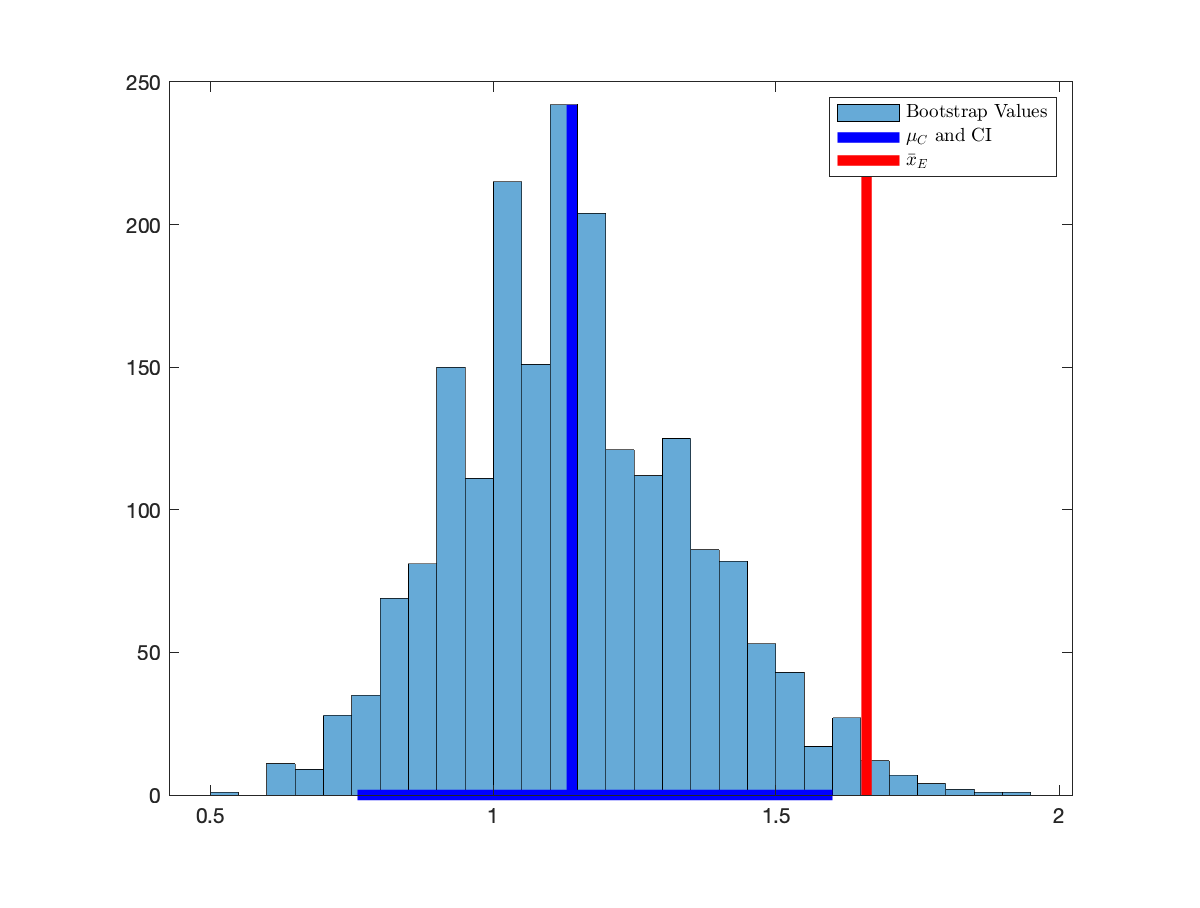
\includegraphics[scale=0.55]{bootstrapOneSample}
\caption{
Histograms of the means of the control bootstrap samples are displayed with the mean of the experimental data  as well as the approximate 95\% confidence interval for the location of the mean of the population that the  control data was sampled from. The means of the experimental samples fall well outside the theoretical confidence intervals.\label{F:bootstrapOneSample}}
\end{figure}
We can see that the experimental mean falls outside the theoretical confidence interval, but just barely. This result contradicts that of the one sample t test, but only very weakly.

A second bootstrap approach for investigating differences between the experimental and control means is to construct bootstrap samples from our experimental and control data and test for differences between \textsl{their} means by computing the achieved significance level (ASL). This will serve in place of a p-value, but it also provides us with a synthetic way of establishing confidence intervals for both our experimental and control means that will give us some indication of range of possible results for our experiment if we were to have replicated it multiple times. We constructed 2000 bootstrap samples each from our control and experimental data sets by repeatedly sampling 100 values from them \textsl{with replacement}. We tracked the mean and standard deviation of these samples so that we could compute a t statistic for each pair of bootstrap samples. We found the ASL by computing the percentage of these t statistics that were larger than the true t statistic computed from our original experimental and control data sets. This resulted in a value of $ASL=0.0725$. This does not fall below 5\%, so it provides no evidence that there is a difference between our experimental and control means. Moreover, we can estimate a pair of 95\% confidence intervals for predicting the location of the means of the populations our experimental and control data were sampled from by computing the 97.5\% and 2.5\% quantiles of the two bootstrap samples. We've displayed these confidence intervals, together with the means of the experimental and control data sets on top of the histograms of the experimental and control bootstrap samples in figure \ref{F:bootstrapTwoSample}.
\begin{figure}[H]
\centering
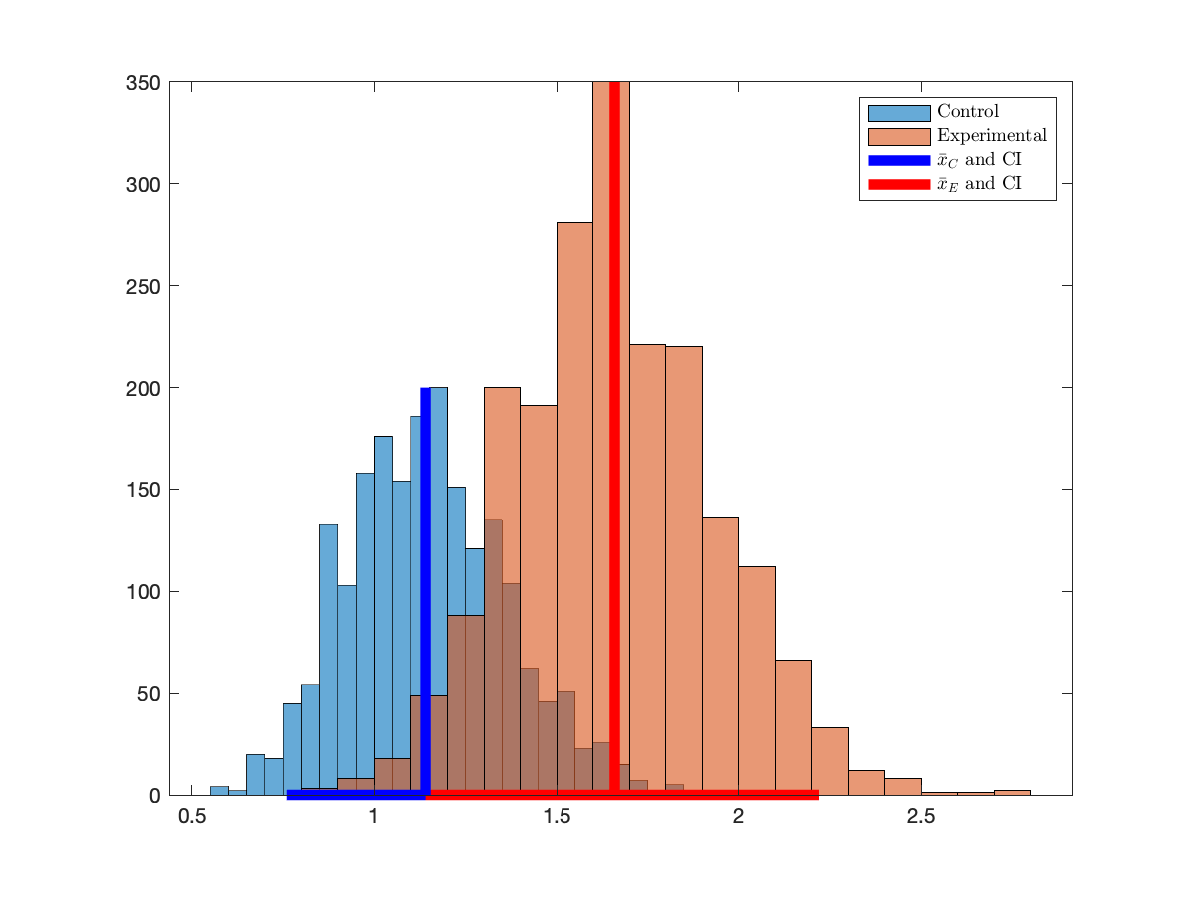
\includegraphics[scale=0.55]{bootstrapTwoSample}
\caption{
Histograms of experimental and control bootstrap samples are displayed with the means of the experimental and control samples as well as the approximate 95\% confidence intervals for the location of the means of the populations that the experimental and control data were sampled from. The experimental mean falls outside the control confidence interval and that the control mean falls outside of the experimental confidence interval.\label{F:bootstrapTwoSample}}
\end{figure}
The fact that the experimental mean falls outside the control confidence interval and that the control mean falls outside of the experimental confidence interval indicates that it is likely that replication of this experiment would reproduce our significant result with great consistency.

In an overall sense, the strongest conclusion we can draw from our various hypothesis tests is that there is inclusive evidence to weak evidence in favor of the notion that normal cholesterol levels are associated with a reduced risk for heart disease. However, the only times we achieved significant results, the significance was rather weak and the competing insignificant results were much more prevalent. A more conservative conclusion for us to draw would be that our experiment produced insufficient evidence for the notion that normal cholesterol levels are associated with a reduced risk for heart disease.
\section{Conclusion}
In this initial study, we were interested in determining whether we could find evidence consistent with the hypothesis that there is a difference in the risk of heart disease when comparing test subjects who have normal cholesterol to test subjects with high cholesterol. We fit a geometric model to the high cholesterol control data set, and performed the geometric test, one sample t test, two sample t test, and bootstrap tests for evaluating differences between the experimental and theoretical mean as well as differences between the means of the experimental and control data. our experiment produced insufficient evidence for the notion that  normal cholesterol levels are associated with a reduced risk for heart disease.\end{document}
